%!TEX root = ../thesis.tex
%*******************************************************************************
%**************************** Introduction Chapter *****************************
%*******************************************************************************
\cleardoublepage
\chapter*{Introduction}
\addcontentsline{toc}{chapter}{Introduction}
\chaptermark{Introduction}
%********************************** %First Section  **************************************


%============================================================%
%============================================================%
\section*{Industrial context and motivation}
%============================================================%
%============================================================%

The current challenge of energy transition involves, among other things, reducing the share of fossil fuels in the global electricity mix. 
In this context, offshore wind energy offers several advantages \citep{eolien_en_mer_2022}. 
Offshore energy benefits from more consistent winds than onshore, mainly due to the absence of terrain roughness, it also makes possible the installation of larger and more powerful wind turbines. 
Since the construction of the first offshore wind farm in Vindeby, Denmark, in 1991, the industry has experienced rapid growth, with a total capacity of 56 GW in operation worldwide in 2021. 
Over time, offshore wind technology has matured, resulting in significant achievements such as securing projects in Europe through ``zero-subsidy bids'' where the electricity produced is directly sold on the wholesale market \citep{eolien_en_mer_2022}. 

However, despite the progress of this sector, scaling limitations and numerous scientific challenges emerge. 
To meet ambitious national and regional development targets, the wind energy industry must address various scaling issues, including port logistics, the demand for critical natural resources, and sustainable end-of-life processes. 
Furthermore, the field presents several scientific challenges that often involve coupling data with numerical simulations of physical systems and their surrounding environment. 
The wind energy community is focused on different objectives, including enhancing the design of floating offshore wind turbines, refining wind resource estimation techniques, and optimizing maintenance operations. 
In general, several decisions are made throughout the lifespan of a wind turbine by its designer, installer, and operator, all while having only partial knowledge of certain physical phenomena. 
Therefore, modeling and controlling the various sources of uncertainties associated with offshore wind energy proved to be a key success factor in this highly competitive industry.
%The design of an offshore wind farm depends on multiple site parameters such as the water depth, soil properties, wind, waves and current conditions, and the local community acceptance. 
%Fortunately, international standards regulate this activity and provide general engineering guidelines. 

Overall, the offshore wind industry needs methods for uncertainty management regarding safety margins and industrial asset management (at the component, wind turbine, and overall wind farm levels) \citep{OWT_review_2016}. 
For wind project developers, the primary focus is on improving the wind potential assessment of candidate sites by combining various sources of information and modeling the multivariate distribution of environmental conditions. 
In the case of floating wind projects, the goal is to incorporate a probabilistic aspect from the design phase (e.g., of the floaters) to define safer, more robust, and more cost-effective solutions.
For wind farm owners, end-of-life management is another significant concern. 
An owner of a wind farm at the end of its life has three options: extend the operational life of assets, replace current wind turbines with newer models, or decommission and sell the wind farm. 
The first two options require evaluating the structural reliability and residual lifespan, with quantitative assessments reviewed by certification bodies and insurers to issue operating permits. 
To provide rigorous risk assessments, the generic methodology of \textit{uncertainty quantification methodology} is a widely accepted approach in industrial sectors facing these types of issues \citep{rocquigny_2008,blanchard_2023}.



%============================================================%
%============================================================%
\section*{Generic methodology for uncertainty quantification} 
%============================================================%
%============================================================%

Computer experiment is a discipline that emerged with the advent of informatics. 
This practice produces numerical models that allow the simulation of complex system behavior based on initial conditions defined by the analyst. 
Numerical models quickly became essential for the analysis, design, and certification of complex systems in cases where experiments or physical measurements are too costly or even unfeasible. 
However, such numerical models are mostly deterministic: the reproducible result of a simulation is associated with a fixed input set of parameters. 
The issue of managing uncertainties associated with these inputs arises when performing analysis with numerical models. 

Uncertainty quantification aims at modeling and controlling uncertainties around a numerical model. 
To do so, a generic methodology has been proposed to quantify and analyze uncertainties between input and output variables of a numerical model \citep{rocquigny_2008,blanchard_2023}. 
An overview of the mathematical tools used in this field is provided by \citet{sullivan_2015}. 
This approach improves the understanding of a system, ultimately contributing to more robust decision-making. 
Figure \ref{fig:UQ_methodo} illustrates the main steps of the generic uncertainty quantification method, which are briefly summarized hereafter: 
\begin{itemize}
    \item \textbf{Step A -- Problem specification}:     
    This step involves identifying the system under study and constructing a numerical model capable of precisely simulating its behavior. 
    Specifying the problem also involves the definition of a set of parameters inherent to the numerical model. 
    These parameters include both the input variables and the output variables generated by the simulation. 
    In this document, the numerical model is considered a black box, in contrast to approaches that are integrated within the numerical solution schemes for the system's behavioral equations (referred to as intrusive approaches \citep{lemaitre_2010}). 
    Generally, these numerical models are first calibrated against measured data and pass a process of validation and verification to reduce modeling errors (see e.g., \citep{oberkampf_2010_VVUQ,damblin_2015,carmassi_2018}.  
    \item \textbf{Step B -- Uncertainty modeling}: 
    The objective of the second step is to identify and model all the sources of uncertainty related to the input variables. 
    Most of the time the uncertainty modeling is done in the probabilistic framework.
    \item \textbf{Step C -- Uncertainty propagation}:
    This step consists of propagating the uncertain inputs through the computer model.  
    Consequently, the output of the numerical model (commonly scalar) also becomes uncertain. 
    The goal is to estimate a quantity of interest, which is a statistic related to the studied random output variable. 
    The uncertainty propagation method may differ depending on the quantity of interest targeted (e.g., central tendency, a quantile, a rare event probability, etc.).    
    \item \textbf{Step C' -- Inverse analysis}: 
    In this additional step, a sensitivity analysis can be performed to study the role allocated to each uncertain input leading to the uncertain output. 
    \item \textbf{Metamodeling}: 
    Considering the high computational cost associated with some simulations, statistical approaches emulate these expensive simulators with a limited number of simulations. 
    Uncertainty quantification can then be carried out using a ``surrogate model'' (or metamodel) for a reduced computational cost. 
    This optional step of statistical learning is not strictly a part of uncertainty quantification, but it often proves to be essential for enabling its practical implementation.
\end{itemize}


\begin{figure}[!h]
    \centering
    %\begin{figure}[h]
%    \centering
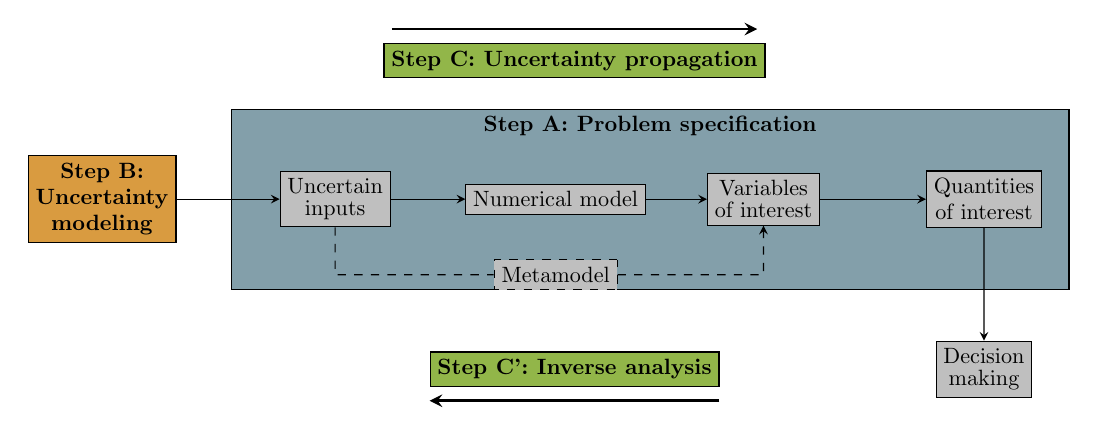
\begin{tikzpicture}[scale=0.8, every node/.style={transform shape}]
    \node[rectangle,draw,fill=YellowOrange!70!gray] (a) at (-9,0) {\shortstack{\textbf{Step B:} \\ \textbf{Uncertainty} \\ \textbf{modeling}}};
\node[rectangle,draw,fill=YellowGreen!70!gray] (f) at (-1.5,2.2) {
\textbf{Step C: Uncertainty propagation}};
\node[rectangle,draw,fill=YellowGreen!70!gray] (g) at (-1.5,-2.7) {\shortstack{
\textbf{Step C': Inverse analysis}}};
\node[rectangle,draw,minimum width=13.3cm,fill=SkyBlue!40!gray] (h) at (-0.3,0) {\shortstack{\textbf{Step A: Problem specification} \\ \phantom{a} \\ \phantom{a} \\ \phantom{a} \\ \phantom{a} \\ \phantom{a} \\ \phantom{a} \\ \phantom{a} \\ \phantom{a} \\ \phantom{a} }};
\node[rectangle,draw,fill=lightgray] (b) at (-5.3,0) {\shortstack{
Uncertain\\ inputs}};
\node[rectangle,draw,fill=lightgray] (c) at (-1.8,0) {\shortstack{
    Numerical model}};
\node[rectangle,draw,fill=lightgray] (d) at (1.5,0) {\shortstack{
Variables \\ of interest}};
\node[rectangle,draw,fill=lightgray] (e) at (5,0) {\shortstack{
Quantities \\ of interest}};
\node[rectangle,draw,fill=lightgray, dashed] (i) at (-1.8,-1.2) {Metamodel};
\node[rectangle,draw,fill=lightgray] (j) at (5,-2.7) {\shortstack{Decision \\ making}};
\draw[-stealth, black, line width=1pt] (-4.4,2.7) -- (1.4,2.7);
\draw[-stealth, black, line width=1pt] (0.8,-3.2) -- (-3.8,-3.2);
\draw[-stealth, black] (a) -- (b);
\draw[-stealth, black] (b) -- (c);
\draw[-stealth, black] (c) -- (d);
\draw[-stealth, black] (d) -- (e);
\draw[-stealth, black, dashed] (b) -- (-5.3,-1.2) -- (i) -- (1.5,-1.2) -- (d);
 \draw[-stealth, black] (e) -- (j);

\end{tikzpicture}
%    \caption{General uncertainty quantification and propagation framework}
%    \label{Fig:UQ}
%\end{figure}
    \caption{General uncertainty quantification framework (\cite{rocquigny_2008}, adapted by \cite{ajenjo_2023})}
    \label{fig:UQ_methodo}
\end{figure}


%============================================================%
%============================================================%
\section*{Problem statement and outline of the thesis}
%============================================================%
%============================================================%

Risk and uncertainty management in the field of wind energy is a significant concern for the electric utility Électricité de France (EDF). 
This thesis aims to adapt and apply the generic uncertainty quantification methodology to industrial offshore wind energy studies. 
As such, this use case raises scientific challenges related to its specific characteristics, described in the following:
\begin{itemize}
    \item The numerical model exploited in the present work consists of a series of numerical models executed sequentially. 
    This chain is divided into three parts: first, a temporal and stochastic generation of wind and wave velocity fields, 
    followed by the simulation of the coupled hydro-aero-servo-elastic behavior of the wind turbine, 
    and finally a post-processing phase to obtain scalar quantities of interest, aggregated over the temporal outputs. 
    \item The complexity of this simulator, along with the high unit computational cost (about 40 minutes per simulation), requires the use of efficient sampling methods and high-performance computing systems. 
    In addition to the complexity associated with the numerical model, modeling the input uncertainties also represents a challenge. 
    Indeed, the joint distribution associated with environmental conditions presents a complex dependence structure.   
    The quality of the inference step is critical as it directly impacts the conclusions of uncertainty propagation.
\end{itemize}

In order to apply the generic methodology for uncertainty quantification to the offshore wind turbine case, this thesis aims to answer the following questions: 
\begin{itemize}
    \item[\textbf{Q1.}] \textit{
    How to accurately model the dependence structure associated with the joint environmental distribution? 
    } (\ding{238} Step B)
    \item[\textbf{Q2.}] \textit{
    How to perform uncertainty propagation through a computationally expensive numerical chain uniquely based on an empirical description (measured data) of input uncertainties?
    } (\ding{238} Step C)
    \item[\textbf{Q3.}] \textit{
    How to estimate rare event probabilities related to the fatigue failure of offshore wind turbine structures?
    } (\ding{238} Step C)
    \item[\textbf{Q4.}] \textit{
    How to assess and analyze the sensitivity of uncertain inputs regarding quantities of interest resulting from structural reliability (i.e., reliability-oriented sensitivity analysis)? 
    } (\ding{238} Step C')
\end{itemize}

To propose an answer to these questions, this manuscript is divided into three parts. 
The first part offers an introduction to uncertainty quantification methods and offshore wind turbine numerical modeling. 
The second part presents the contributions of this thesis to uncertainty quantification and propagation while the third part describes the contributions to rare event estimation. 
This manuscript is divided into seven chapters, which are summarized hereafter: 

\paragraph{Chapter 1 -- Introduction to uncertainty quantification.} 
%------------------------------------------------------------%
This chapter gives a brief overview of various topics in uncertainty quantification \citep{sullivan_2015}. 
After a reminder of some mathematical concepts, the model specification step is described, considering a black box and its input and output variables. 
The different types and sources of uncertainties are then presented, along with their modeling within a probabilistic framework. 
Uncertainty propagation depends on the estimated quantities of interest, therefore, one section addresses propagation methods for central tendency studies, 
and another focuses on rare event probability estimation (a statistic related to the tails of output distributions). 
The section dedicated to central tendency presents numerical integration, sampling, and design of experiment methods \citep{fang_liu_2018}. 
The one about rare event probabilities introduces usual methods from the field of structural reliability \citep{lemaire_2009,MorioBalesdent2015}. 

This chapter also covers the main methods for global sensitivity analysis \citep{daveiga_iooss_2021}. 
This field divides its methods into two major classes: screening methods and importance measures. 
Screening techniques typically applied in high-dimensional problems, aim to identify variables with low impact on the variability of the output of interest. 
Importance measures, on the other hand, quantitatively allocate, for each input variable, a share of the output variability, enabling the ranking of variables based on their influence.

Finally, this chapter presents an overview of the families of metamodels commonly used in uncertainty quantification \citep{forrester_2008}. 
Special attention is given to the Gaussian process regression, which involves conditioning a Gaussian process on a set of observations from the numerical model. 
Once conditioned, the Gaussian process provides richer information than other types of metamodels. 
This method simultaneously offers a surrogate model (mean of the Gaussian process, also called predictor) and an error function (variance of the process). 
Some iterative methods (called ``active'') use this additional information to progressively enrich the metamodel and improve its predictability. 
These techniques were quite successful in the 1990s for solving optimization problems with expensive functions \citep{jones_1998}. 
Since then, their use has expanded to solve problems in structural reliability \cite{echard_2011}.


\paragraph{Chapter 2 -- Introduction to wind turbine modeling and design.} 
%------------------------------------------------------------%
The simulation of an offshore wind turbine involves modeling multiple physical aspects interacting with random environmental conditions. 
This chapter first introduces spectral methods used to generate wind and wave velocity fields by applying inverse Fourier transforms (e.g., as implemented in the TurbSim tool \citep{turbsim_2009}]). 
These simulated wind velocity fields then become the inputs of a multi-physics wind turbine numerical model. 
Such simulation includes simplified modeling of the interactions between fluids and structures (using the blade element momentum theory), dynamic modeling of the structure using flexible multibody methods, and modeling of wind turbine control systems [source]. 
The numerical code studied generates a time series of several physical quantities describing the system's behavior.

This thesis particularly focuses on the probabilistic evaluation of fatigue damage in wind turbine structures. 
Fatigue damage is a phenomenon that deteriorates the mechanical properties of a material as a result of exposure to many cyclic low-amplitude stresses. 
Currently, standards recommend the use of deterministic safety factors to address this failure mode \citep{iec_2019,dnv_loads_2016}. 
A probabilistic approach enhances the analysis and can sometimes reveal conservative safety margins. 
Several recent studies have addressed this topic from different methodological perspectives \citep{huchet_2019,lataniotis_2019,cousin_2021,hirvoas_2021,petrovska_2022}.

In this context, this chapter enumerates the input parameters of the calculation chain that are considered uncertain. 
These random variables are grouped into two groups: the random vector related to the environment (e.g., average wind speed, wind speed standard deviation, wind direction, significant wave height, wave period, and wave direction), 
and the random vector related to the system (e.g., controller wind misalignment error, soil stiffness, fatigue calculation curve parameters).


\paragraph{Chapter 3 -- Kernel-based uncertainty quantification.} 
%------------------------------------------------------------%
This chapter examines perturbations in environmental conditions within an offshore wind farm induced by wake effects \cite{larsen_2008_wake}. 
A theoretical offshore wind farm off the southern coast of Brittany is considered as a use case, and a simplified numerical model of wake in this wind farm is used. 
This model provides an analytical prediction of the wind speed deficit and turbulence created by the wake, taking into account the influence of the floaters' positions due to rigid body dynamics. 

In the second phase, uncertainty propagation is carried out through the wake model, considering the joint distribution of ambient environmental conditions as inputs. 
In the end, an environmental distribution perturbed by the wake is simulated for each wind turbine. 
A dissimilarity measure between distributions, based on kernels and named the \textit{maximum mean discrepancy} (MMD), is used to compare the distributions perceived by each wind turbine. 
This measure allows the clustering of wind turbines exposed to similar environmental conditions, resulting in identical structural responses. 
Given the high computational cost of aero-servo-hydro-elastic simulations for offshore wind turbines, this preliminary study enables reliability analysis at the wind farm scale without repeating the analysis for each turbine. 
Ultimately, only four classes are selected to represent a wind farm of 25 turbines.


\paragraph{Chapter 4 -- Kernel-based central tendency estimation.} 
%------------------------------------------------------------%
Chapter four presents the use of the kernel-based dissimilarity measure (MMD) in the context of probability distribution sampling, a method known as "kernel herding" introduced by \citet{chen_welling_2010}. 
This quadrature technique belongs to the family of "Bayesian quadratures" \citet{briol_oates_2019}, which can be viewed as a generalization of quasi-Monte Carlo methods \citet{hickernell_2020}. 

The properties of this method are highlighted through an industrial application dedicated to estimating the mean fatigue damage of a wind turbine structure. 
Although this quantity is crucial in the design and certification of wind turbines, the methods used to estimate it are known to be suboptimal (i.e., regular grids). 
The study is conducted on a model of a fixed offshore wind turbine belonging to a farm in the North Sea. 
Uncertainties in input environmental conditions are inferred from in-situ measured data. 

Finally, a numerical comparison with Monte Carlo and quasi-Monte Carlo sampling reveals the performance and practical advantages of kernel herding. 
This method allows for direct subsampling from a large environmental database without the need for inference (step B).


\paragraph{Chapter 5 -- Kernel-based metamodel validation.} 
%------------------------------------------------------------%
This chapter proposes the use of kernel-based sampling methods in the context of model validation for machine learning (or surrogate models). 
Estimating the predictivity of supervised learning models requires an evaluation of the learned surrogate model on a set of test points that were not used during training. 
The quality of the validation naturally depends on the properties of the test set and the metric used to summarize the prediction error. 
This contribution first suggests using space-filling sampling methods to ``optimally'' select a test set, then, 
it introduces a new predictivity coefficient that weights the observed errors to improve the global error estimation. 
A numerical comparison between several sampling methods based on geometric approaches \citep{shang_apley_2020} or kernel methods \cite{chen_welling_2010,mak_joseph_2018} is carried out. 
Our results show that weighted versions of kernel methods offer superior performance. 
An application to simulated mechanical loads in an offshore wind turbine model is also presented. 
This experiment illustrates the practical relevance of this technique as an effective alternative to costly cross-validation techniques.

\paragraph{Chapter 6 -- Nonparametric rare event estimation.} 
%------------------------------------------------------------%
Estimating rare event probabilities is a common issue in industrial risk management, especially in the field of structural reliability \citep{chabridon_2018_thesis}. 
To address this, several techniques have been proposed to overcome the known limitations of the Monte Carlo method. 
Among them, ``subset simulation'' \citep{AuBeck2001} is a technique based on the split of a rare probability into a product of less rare (and thus easier to estimate) conditional probabilities associated with nested failure events. 
However, this technique relies on conditional simulation using Markov chain Monte Carlo (MCMC) methods. 
These algorithms, while converging, often produce samples that are not independent and identically distributed (i.i.d.) due to the correlation between the Markov chains.
In this chapter, another conditional sampling method is proposed, with the advantage of preserving the i.i.d. property. 
Independent sampling is particularly relevant for reusing these samples in a posterior reliability-oriented sensitivity analysis. 
The algorithm introduced is based on the non-parametric inference of the conditional joint distribution using kernel density estimation of marginals combined with dependence inference using the empirical Bernstein copula \citep{sancetta_satchell_2004}. 
The so-called ``Bernstein adaptive nonparametric conditional sampling'' (BANCS), is compared to the subset simulation method for several structural reliability problems. 
The initial results are promising, but further investigation is needed to control the estimator's bias.


\paragraph{Chapter 7 -- Sequential reliability oriented sensitivity analysis.} 
%------------------------------------------------------------%
This chapter deals with sensitivity analysis for risk measures (e.g., rare event probabilities). 
Global sensitivity analysis \citep{daveiga_iooss_2021} assigns a portion of the global output variability to each variable (or group of variables), often using a functional decomposition of the output variance. 
However, when studying risk measures (often located in the distributions' tails), the global sensitivity might be very different from the sensitivity to the risk measure. 
``Reliability-oriented sensitivity analysis'' (\abv{rosa}), studies the impact of the inputs in regard to a risk measure such as a rare event probability (see e.g., \citet{chabridon_2018_thesis}). 
Using the nested subsets obtained with the BANCS algorithm (presented in Chapter 6), the idea of this chapter is to study the ROSA evolution as the subsets get closer to the failure domain. 
For each subset, a ROSA is carried out with a kernel-based importance measure called the ``Hilbert-Schmidt Independence Criterion'' adapted to this context \citep{marrel_chabridon_2021}. 

\clearpage
%============================================================%
%============================================================%
\section*{Numerical developments}
%============================================================%
%============================================================%

Several implementations developed in this thesis are available on different platforms, allowing the reader to reproduce some numerical results in an open-data approach:  

\begin{center}
\footnotesize
\begin{tabularx}{\textwidth}{l >{\raggedleft\arraybackslash}X}
    \texttt{\href{https://efekhari27.github.io/otkerneldesign/master/}{otkerneldesign}}\footnotemark
    &    
    \begin{itemize}[left=0pt]
        \item This Python package generates designs of experiments based on kernel methods such as Kernel Herding and Support Points. 
        A tensorized implementation of the algorithms was proposed, significantly increasing their performances. 
        Additionally, optimal weights for Bayesian quadrature are provided. 
        \item This Python package, developed in collaboration with J.Muré, is available on the platform Pypi and fully documented.
    \end{itemize}\\ \hline
    \texttt{\href{https://github.com/efekhari27/bancs}{bancs}}\footnotemark &    
    \begin{itemize}[left=0pt]
        \item This Python package proposes an implementation of the ``Bernstein Adaptive Nonparametric Conditional Sampling'' method for rare event estimation. 
        \item This Python package is available on the PyPI platform and is illustrated with examples and analytical benchmarks.
    \end{itemize}\\ \hline
    \texttt{\href{https://github.com/efekhari27/ctbenchmark}{ctbenchmark}}\footnotemark &    
    \begin{itemize}[left=0pt]
        \item This Python package presents a standardized process to benchmark different sampling methods for central tendency estimation. 
        \item This Python package is available on a GitHub repository with analytical benchmarks.
    \end{itemize}\\ \hline
    \href{https://github.com/efekhari27/copulogram}{\texttt{copulogram}}\footnotemark &    
    \begin{itemize}[left=0pt]
        \item This Python package proposes an implementation of a synthetic visualization tool for multivariate distributions. 
        \item This Python package, developed in collaboration with V.Chabridon, is available on the Pypi platform.
    \end{itemize}\\
\end{tabularx} 
\end{center}

\footnotetext[1]{Documentation: \url{https://efekhari27.github.io/otkerneldesign/master/}}
\footnotetext[2]{Repository: \url{https://github.com/efekhari27/bancs}}
\footnotetext[3]{Repository: \url{https://github.com/efekhari27/ctbenchmark}}
\footnotetext[4]{Repository: \url{https://github.com/efekhari27/copulogram}}

\newpage
%============================================================%
%============================================================%
\section*{Publications and communications}
%============================================================%
%============================================================%

The research contributions in this manuscript are based on the following publications: 

\begin{center}
    \footnotesize
    \renewcommand*{\arraystretch}{1.4}
    \begin{tabularx}{\textwidth}{c X}
        Book Chap.      & \underline{E. Fekhari}, B. Iooss, J. Muré, L. Pronzato and M.J. Rendas (2023). 
                        ``Model predictivity assessment: incremental test-set selection and accuracy evaluation''. 
                        In: \textit{Studies in Theoretical and Applied Statistics}, pages 315--347. Springer.\\
        \hline  
        Jour. Pap.      & \underline{E. Fekhari}, V. Chabridon, J. Muré and B. Iooss (2023).
                        ``Given-data probabilistic fatigue assessment for offshore wind turbines using Bayesian quadrature''. 
                        In: \textit{Data-Centric Engineering}.\\

                        %& \elias{\underline{E. Fekhari}, V. Chabridon, J. Muré and B. Iooss (2023).
                        %``TO DO: Bernstein adaptive nonparametric conditional sampling''.
                        %In: \textit{Special Issue in Honor of Professor Armen Der Kiureghian. Reliability Engineering \& System Safety}.}\\
        \hline
\shortstack{Int. Conf.\\Pap.}& \underline{E. Fekhari}, B. Iooss, V. Chabridon, J. Muré (2022). 
                    ``Efficient techniques for fast uncertainty propagation in an offshore wind turbine multi-physics simulation tool''.
                    In: \textit{Proceedings of the 5th International Conference on Renewable Energies Offshore (RENEW 2022)}, Lisbon, Portugal. (Paper \& Talk)\\
        
                    & \underline{E. Fekhari}, V. Chabridon, J. Muré and B. Iooss (2023). 
                    ``Bernstein adaptive nonparametric conditional sampling: a new method for rare event probability estimation''\footnote{This contribution was rewarded by the ``CERRA Student Recognition Award''}.
                    In: \textit{Proceedings of the 13th International Conference on Applications of Statistics and Probability in Civil Engineering (ICASP 14)}, Dublin, Ireland. (Paper \& Talk)\\
        
                    & E. Vanem, \underline{E. Fekhari}, N. Dimitrov, M. Kelly, A. Cousin and M. Guiton (2023). 
                    ``A joint probability distribution model for multivariate wind and wave conditions''.
                    In: \textit{Proceedings of the ASME 2023 42th International Conference on Ocean, Offshore and Arctic Engineering (OMAE 2023)}, Melbourne, Australia. (Paper)\\
        
                    & A. Lovera, \underline{E. Fekhari}, B. Jézéquel, M. Dupoiron, M. Guiton and E. Ardillon (2023). 
                    ``Quantifying and clustering the wake-induced perturbations within a wind farm for load analysis". 
                    In: \textit{Journal of Physics: Conference Series (WAKE 2023)}, Visby, Sweden (Paper)\\
        \hline
\shortstack{Int. Conf.\\Short Abs.}  & \underline{E. Fekhari}, B. Iooss, V. Chabridon, J. Muré (2022).
                    ``Numerical Studies of Bayesian Quadrature Applied to Offshore Wind Turbine Load Estimation''.
                    In: \textit{SIAM Conference on Uncertainty Quantification (SIAM UQ22)}, Atlanta, USA. (Talk)\\
        
                    & \underline{E. Fekhari}, B. Iooss, V. Chabridon, J. Muré (2022). 
                    ``Model predictivity assessment: incremental test-set selection and accuracy evaluation''.
                    In: \textit{22nd Annual Conference of the European Network for Business and Industrial Statistics (ENBIS 2022)}, Trondheim, Norway. (Talk)\\
        \hline
        Nat. Conf.  & \underline{E. Fekhari}, B. Iooss, V. Chabridon, J. Muré (2022).
                    ``Kernel-based quadrature applied to offshore wind turbine damage estimation''. 
                    In: \textit{Proceedings of the Mascot-Num 2022 Annual Conference (MASCOT NUM 2022)}, Clermont-Ferrand, France (Poster)\\
        
                    & \underline{E. Fekhari}, B. Iooss, V. Chabridon, J. Muré (2023).
                    ``Rare event estimation using nonparametric Bernstein adaptive sampling''. 
                    In: \textit{Proceedings of the Mascot-Num 2023 Annual Conference (MASCOT-NUM 2023)}, Le Croisic, France (Talk)\\
        \hline
        Invited Lec.& Le Printemps de la Recherche 2022, Nantes, France. ``Traitement des incertitudes pour la gestion d’actifs éoliens''. (Talk)\\

                    & Journées Scientifiques de l’Eolien 2024, Saint-Malo, France. ``Evaluation probabiliste de la fiabilité en fatigue des structures éoliennes en mer''. (Talk)
                    
        \end{tabularx}    
\end{center}

